\section{Evaluation}
\label{evaluation}
To be successful, \revenge needs to be able to properly evaluate submitted programs, and the overhead of data collection must not discourage reverse engineers from using the system. We evaluate these issues next.

%%%%%%%%%%%%%%%%%%%%%%%%%%%%%%%%%%%%%%%%%%%%%%%%
\subsection{Correctness analysis}
\begin{figure}[t]
\centering
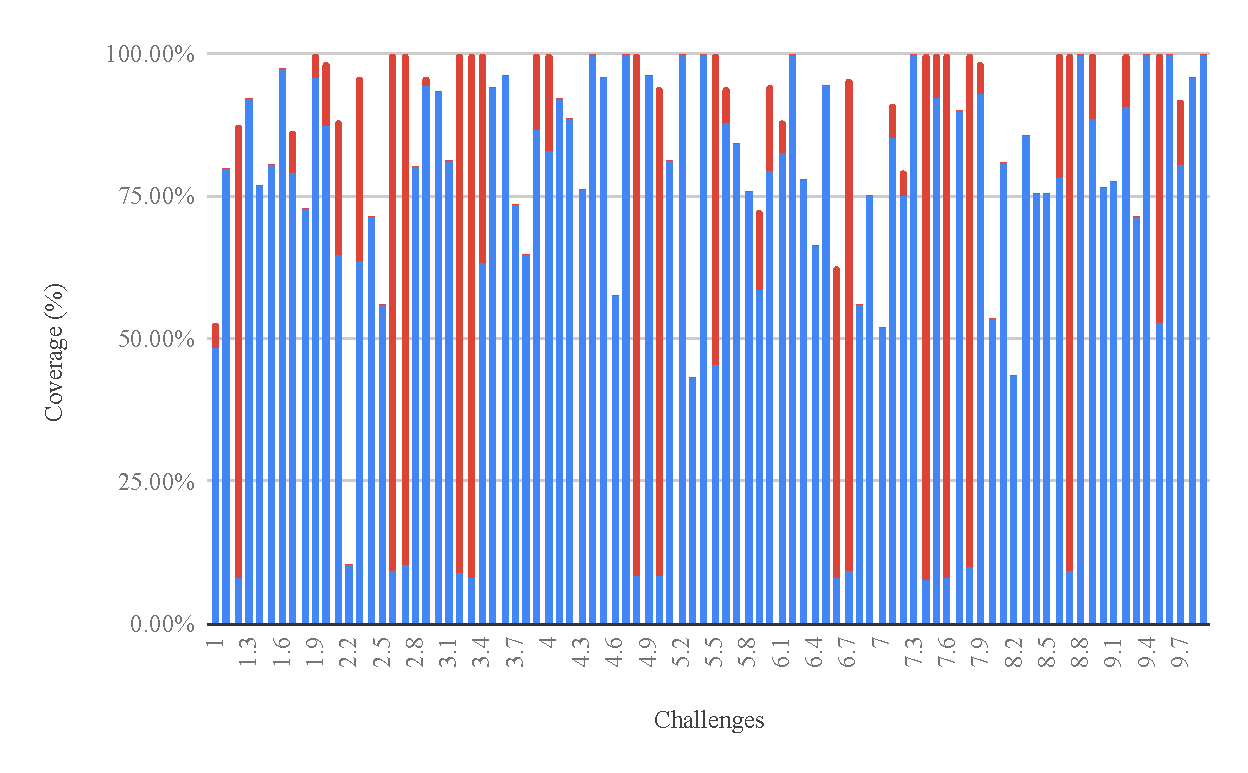
\includegraphics[width=\columnwidth]{coverage.pdf}
\caption{Path coverage (using {\tt gcov}) for generated test cases. Blue bars represent the number of unique test cases contributed by Klee's symbolic analysis, red bars unique test cases contributed by random input generation.}
\label{fig:coverage}
\end{figure}

To determine whether a submitted program in fact solves a challenge, we need to determine that it is equivalent to the original, generated, random program. We use two methods to generate test cases to compare the two programs for equivalence: symbolic analysis using Klee, and random generation from a distribution. Figure~\ref{fig:coverage} shows the path coverage that these methods achieve. 

On average, we achieve 85\% coverage. In the future we will remedy this by a) using multiple symbolic analysis engines which use different search strategies, b) extending symbolic analysis with {\em fuzzing}~\cite{DBLP:conf/ndss/StephensGSDWCSK16}. Currently, when we still fail to achieve 100\% coverage, we re-generate the random challenge program.

%\subsubsection{Precision Analysis}
%Given a submission that is equivalent to the original, it is not yet clear how close performance wise and structurally it must be in order to be considered deobfuscated.  Because the term \textit{deobfuscated} itself is open to interpretation, initial submissions will be liberally auto-graded and the grading model refined as more in depth analysis is done on submissions.

%%%%%%%%%%%%%%%%%%%%%%%%%%%%%%%%%%%%%%%%%%%%%%%%
\subsection{Overhead of data collection}

\revenge's data collection software must be relatively transparent, such that it does not interfere with subjects' ability to reverse engineer.  In our experiments, the data collection occupied about 120\% of a single x86 core CPU and 40\% of 4 GB of memory after executing for about 1.68 days. Figure~\ref{fig:datacollectionperformance} shows an ARM device that was allocated 2 GB of memory and left executing for 1.2 hours reaching 102\% of a single core usage and 20\% of memory usage. The device was significantly laggy---though usable---compared to the x86 virtual machine with additional resources.

%We require that participants run our data collection software in a virtualized environment which records the interaction between the human and the device.  Screenshots and process information are collected on both polling and interrupt bases, with a 15 second sample rate on the polling.  The rest of the data is collected via interrupts only.

%\begin{figure}[t]
%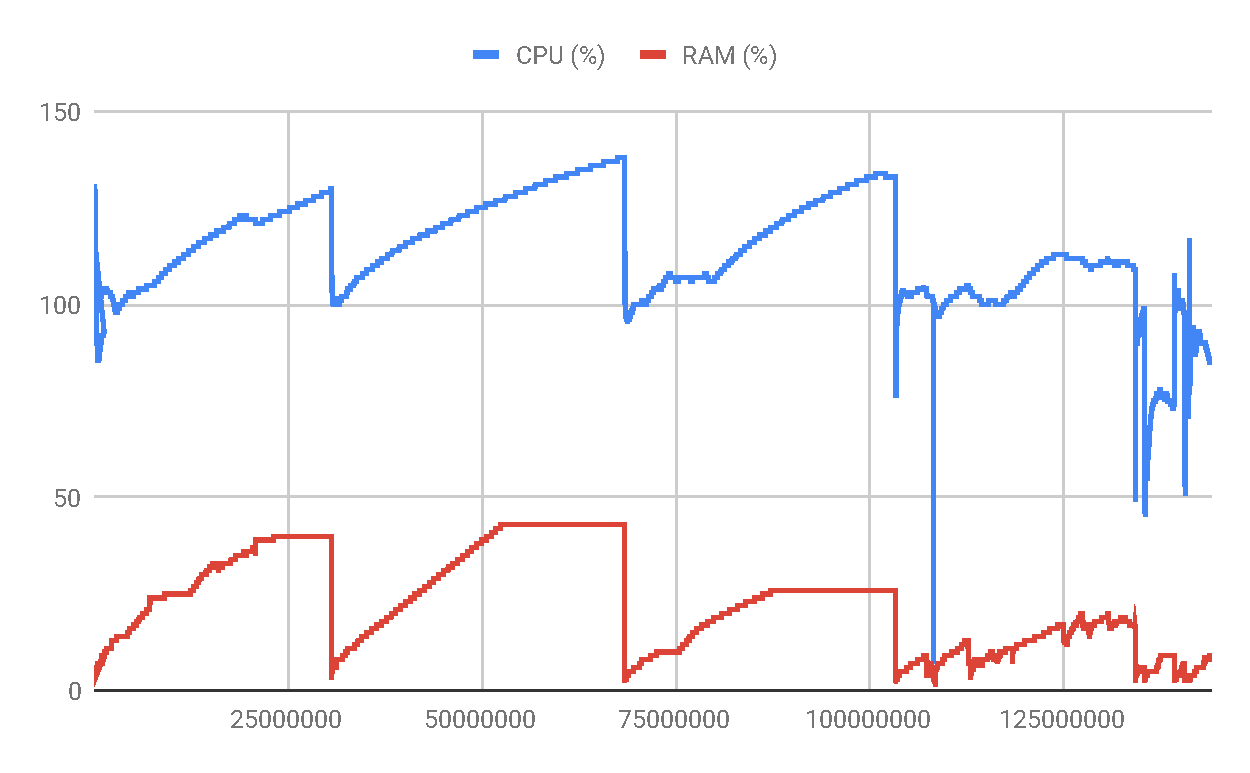
\includegraphics[width=\columnwidth]{datacollectionperformancex86.pdf}
%\caption{CPU and RAM usage for the entirety of the 1.68 day x86 run.}
%\label{fig:datacollectionperformancex86}
%\end{figure}

\begin{figure}[t]
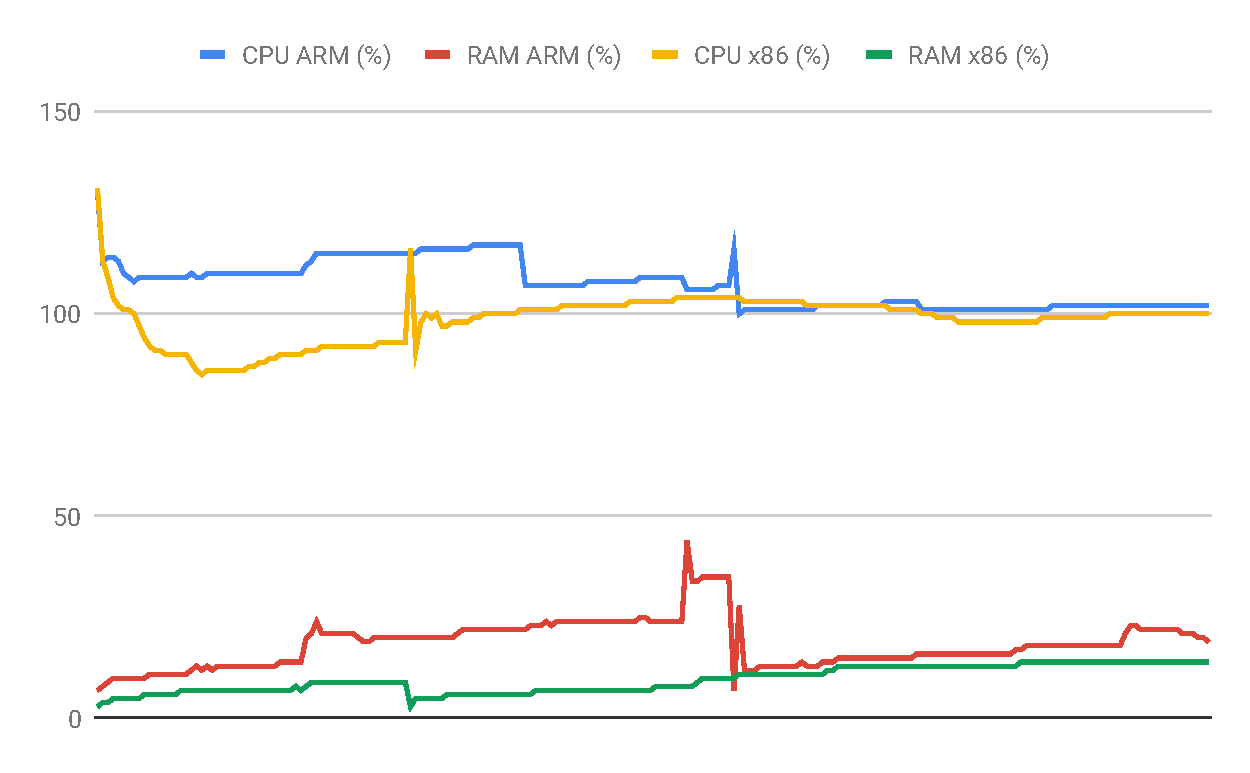
\includegraphics[width=\columnwidth]{datacollectionperformance.pdf}
\caption{CPU and RAM usage for two data collection runs, one on an x86 device and one on an ARM device, both using an Ubuntu virtual machine.}
\label{fig:datacollectionperformance}
\end{figure}

After executing for 1.68 days on a high resolution (1920x1440) display, the initial x86 data collection trial run had accumulated about 1 GB of screenshot data, and another 400 MB of process data---these two polled resources dwarf all other data by at least an order of magnitude.
%If necessary, storage requirements can be reduced by a) lowering the polling rate, b) reducing screen resolution (operating at a 1280x720 resolution, the ARM device accumulated only 29.5MB of screenshots over 1.2 hours), or c) pre-processing the images (by optical character recognition, for example), and storing this data instead of the screenshots themselves. 

%Operating at a more modest 1280x720 resolution, the ARM device accumulated a mere 50 MB of data, of which 29.5 consisted of screenshots and 19.7 process data.

%Given all of this, the data collection software developed for RevEngE appears sound based on testing.  As participants utilize the system, additional evaluation will be done on this component.

%What is the overhead of the data collection framework? How much data is collected over time, as a user performs their task? What is the slowdown of running the collection vs. not?


%\CC{
%\begin{enumerate}
%    \item How well does our correctness analysis work? I.e., what code coverage are we getting on our challenges?
%    \item How well does our precision analysis work (I don't know how to test this, maybe we need to punt).
%    \item What is the overhead of the data collection framework? How much data is collected over time, as a user performs their task? What is the slowdown of running the collection vs. not?
%\item How effective is the data collection framework? I.e., do we collect enough information to perform the analysis? (I don't know how to test this, maybe we need to punt).
%    \item How good is the visualization? (I don't know how to test this, maybe we need to punt).
 %   \item How about including an example of what we collected for a particular de-obfuscation run? A sequence of screenshots (they would have to be small!), process data, window data, etc.
%\end{enumerate}
%}

\endinput

To measure how we Using gcov, we measure exactly how much of the source code was executed as a metric; some code, of course, may not ever possibly be executed (and is dead code) but the metric supplies an idea of how accurate the correctness testing is.

 However, not all code in our programs is necessarily reachable, and there is no guarantee that Klee will find all paths within a reasonable time.  So, we limit the amount of time in order to obtain an approximation of the total edge cases for a program.  Random values are also used to extend coverage further.
 
As shown in Table ~\ref{tab:kleeresults}, even without analysis of dead source code Klee is able to achieve almost 70\% code coverage on all programs.  In some cases, Klee did not produce any results, warranting further investigation.  With these results omitted until such investigation, Klee alone can achieve over 80\% coverage in our configuration on our randomly generated problems.  Adding randomly generated cases increases that to about 85\%, with a sample size of 100 test cases.  We believe this to be sufficient for initial grading aimed to filter extraneous submissions in conjunction with performance analysis doing the same.  More in depth analysis of submissions for correctness may be done if they manage to pass the cases generated, including using Klee or other symbolic execution engines for greater periods of time to generate additional cases.

\begin{table}[]
\caption{Code Coverage Results}
\label{tab:kleeresults}
\begin{tabular}{@{}llll@{}}
\toprule
                     & Klee Cases & Klee + Random & Diff    \\ \midrule
Average Coverage     & 69.23\%    & 85.83\%       & 17.69\% \\
Average w/o Failures & 80.33\%    & 85.19\%       & 4.86\%  \\ \bottomrule
\end{tabular}
\end{table}
\textbf{}